\documentclass[twoside,11pt]{article}

% Any additional packages needed should be included after jmlr2e.
% Note that jmlr2e.sty includes epsfig, amssymb, natbib and graphicx,
% and defines many common macros, such as 'proof' and 'example'.
%
% It also sets the bibliographystyle to plainnat; for more information on
% natbib citation styles, see the natbib documentation, a copy of which
% is archived at http://www.jmlr.org/format/natbib.pdf

\usepackage{jmlr2e}
\usepackage{xcolor}
\usepackage{hyperref}

% Definitions of handy macros can go here

\newcommand{\dataset}{{\cal D}}
\newcommand{\fracpartial}[2]{\frac{\partial #1}{\partial  #2}}

% Heading arguments are {volume}{year}{pages}{submitted}{published}{author-full-names}

%\jmlrheading{1}{2000}{1-48}{4/00}{10/00}{Marina Meil\u{a} and Michael I. Jordan}

% Short headings should be running head and authors last names

%\ShortHeadings{Learning with Mixtures of Trees}{Meil\u{a} and Jordan}
\firstpageno{1}

\begin{document}

\title{Detecting Protest Images on Twitter \\
Using Visual and Natural Language Features}

\author{\name Kyle Shaffer \email shafferk@live.unc.edu \\
       \addr School of Information \& Library Science\\
       University of North Carolina at Chapel Hill\\
       Chapel Hill, NC 27599, USA}

\editor{\textcolor{white}{Leslie Pack Kaelbling}}

\maketitle

\begin{abstract}%   <- trailing '%' for backward compatibility of .sty file
Twitter and other social media platforms have increasingly become a medium for communicating opinions regarding issues of social import. More recently, these platforms have served as a tool for organizing protests and demonstrations in response to developing social issues. This presents both a challenge and an opportunity for news organizations seeking to cover these events as they unfold. In this paper, automated methods are explored for identifying images of protest scenes that are shared on Twitter. A unique dataset of tweets collected by the author is analyzed and used for supervised machine learning experiments to investigate the impact of different combinations of visual and natural language features on predicting the presence or absence of a protest image being shared with a tweet. Labels for these experiments are mined from the text of the tweets, and used as a weak label in order to run the supervised learning experiments. Finally, a feature ablation analysis is presented showing that certain linguistic features greatly aid prediction of images depicting these protest scenes.
\end{abstract}
\begin{keywords}
  Social media, Twitter, text mining, scene recognition
\end{keywords}

\section{Introduction}\label{sec:intro}
Social media platforms have emerged as much more than a way to connect with people or stay in touch with friends. In light of recent events, these social media platforms have been used as a way to shed light on social movements, many of which are begun in response to a perceived injustice or crisis situation. Memorable examples of such usage include the Occupy Wall Street and Arab Spring movements. In both these cases, social media was being used as a way to communicate and share aspects of events to a broader audience, as well as a way to organize these events, many of which centered around protest.
\par
More recently, Twitter in particular has emerged as a prominent platform through which people have organized protests and demonstrations in response to a series of deadly events involving police officers and unarmed African American men. These events throughout the United States have given rise to protests and demonstrations, sparking a hashtag-inspired movement known as \url{#blacklivesmatter}. Many users on Twitter have documented these massive protests through photo-sharing, making this a valuable source of large-scale data to understand how these events are unfolding in real time. However, though this large amount of data is extremely valuable, it is also extremely time consuming to manually examine these tweets individually for interesting content.
\par
In this work, a dataset of tweets was collected pertaining to the announcement of a Grand Jury's decision to not indict an NYPD officer in the case of the death of Staten Island man Eric Garner. Roughly 86,000 image-tweet pairs are used as input data for machine learning classifiers to predict whether a protest scene image is being shared in the photo, given a set of image and natural language features. In addition, a straightforward technique for automatically extracting labels for supervised learning experiments is presented. Finally, the results of these experiments are presented through a feature ablation analysis in order to understand which features are most helpful for these classifiers. Results show that several natural language features are helpful for detecting these images with good performance in terms of average precision.

\section{Description of Dataset}
As mentioned in Section \ref{sec:intro} above, the dataset used in this work contains roughly 86,000 tweets and images which will be used for supervised learning experiments. These tweets and their corresponding images were collected through Twitter's Streaming API\footnote{\url{https://dev.twitter.com/streaming/overview}} from 12/3/2014 (the day of the Grand Jury decision) to 12/10/2014 (one week after the Grand Jury decision). This time span for collecting the tweets was a somewhat arbitrary decision - the main goal was to collect a sizable amount of image and text data over a long enough span of time to ensure some variety in the data.
\par
The originally collected dataset of tweet objects returned by the API was roughly 1.5 million tweets. However, given that this project's goal is to detect the content of images within the dataset, only tweets that were sharing an image were of interest. Additionally, not all tweets with an associated image had an image that was downloadable at the time of the project. That is, many of the tweets that were originally published sharing an image were either deleted or protected prior to the author's attempts to download the images. This pared down the size of the dataset to roughly 170,000 tweets that had associated images that could be downloaded. Of these, 86,000 were selected (slightly more than half the dataset) for running experiments. 

\section{Methods}
In this section, the methods for extracting labels for supervised experiments, as well as evaluation and experimental setup are presented.

\subsection{Extracting Labels}
While there is an ample amount of data for conducting supervised learning experiments, there is an initial problem in that no labels for these experiments are ready-made within the dataset. This necessitates some method of labeling the data in order for supervised learning algorithms to use these in the training stage of the experiments. In the past, often expert annotators have gone through an entire dataset and labeled each instance with an appropriate concept or class. However, as datasets have grown in size, this method has become somewhat infeasible. Many researchers have taken to crowdsourcing methods such as utilizing the Mechanical Turk\footnote{\url{https://www.mturk.com/mturk/welcome}} platform to obtain labels from non-expert annotators cheaply and quickly. Other researchers have investigated methods for automatically labeling data using terms within text associated with their data as a kind of ``weak label'' for classifiers to learn from. \cite{wang2009building}, for instance, developed text-based features for image classification and found these to significantly improve performance in their study. Simlarly, \cite{laptev2008learning} used text features from movie scripts to label and learn human actions within the frames of major films.
\par
These past studies show that classifiers can indeed learn a reasonable signal from labels extracted from text, and a version of this approach is taken for the current work. For the present study, the goal of classifiers is to detect the presence or absence of a protest scene in an image. Each of these images is accompanied by some kind of text in the form of a tweet. Thus, text from these tweets was used to form the labels of presence or absence of a protest image being shared with a particular tweet. In order to extract text that would be useful for identifying these labels, several natural language processing steps were taken. First, the text was cleaned with Twitter-specific punctuation stripped out (e.g. \#, RT, @), and then tokenized. Next, all text was stemmed using a pre-trained stemmer through the Python programming language. Finally, the stems protest*, crowd*, and march* were used as indicators of presence of a protest image, and tweets containing any of these stems had their images added to the positive class for protest images. Roughly 16,000 images were seen to belong to the ``protest'' class using this labeling method. Figures \ref{im:good} and \ref{im:noisy} show examples of reasonable and noisy images respectively labeled as belonging to the ``protest'' class.

\begin{figure}[h]
\centering
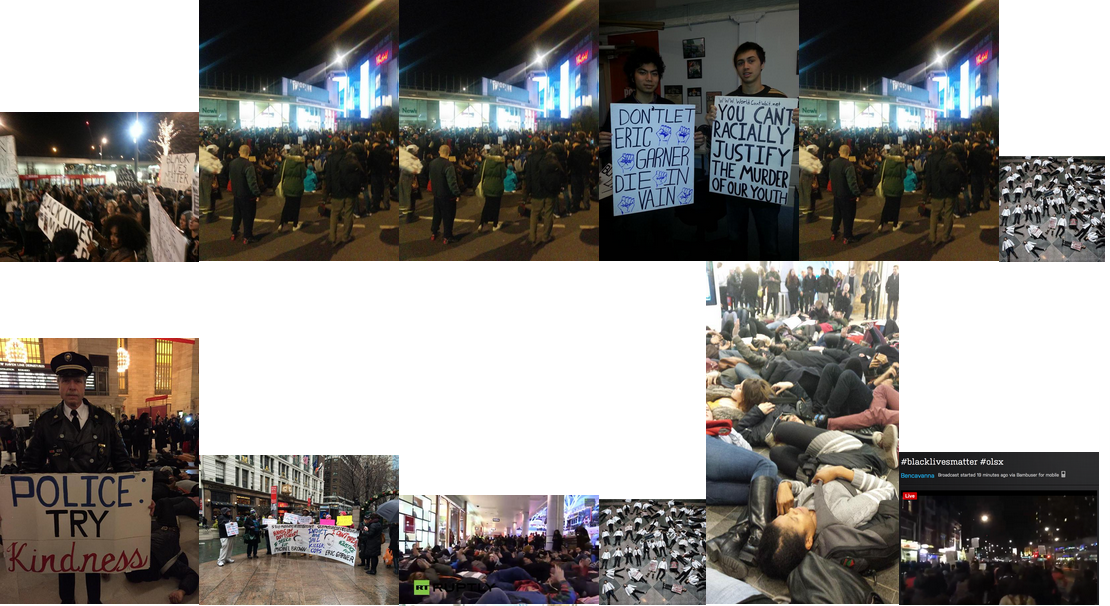
\includegraphics[width=0.75\textwidth]{sample_images_good.png}
\caption{Cohesive examples of images belonging to the protest class using NLP methods to  assign labels.}
\label{im:good}
\end{figure}

\begin{figure}[h]
\centering
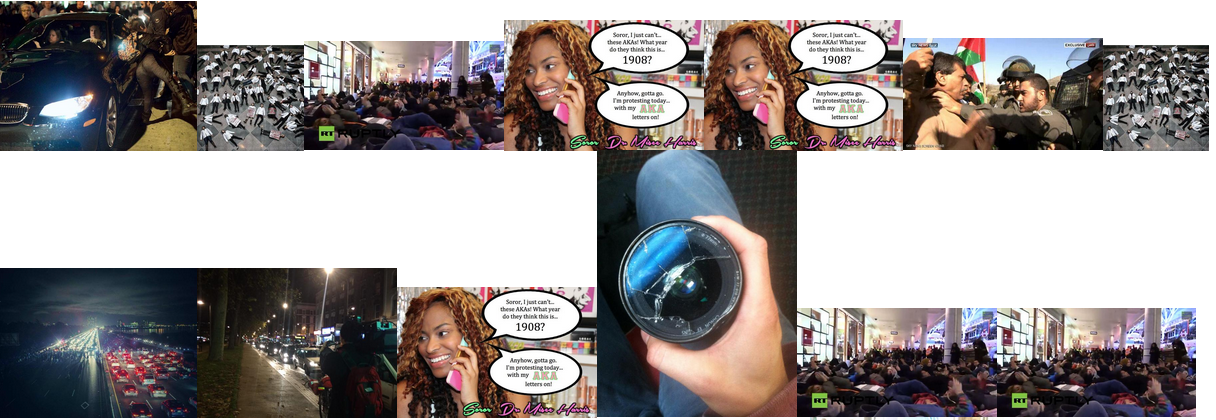
\includegraphics[width=0.75\textwidth]{sample_images_noise.png}
\caption{Noisy images belonging to the protest class using NLP methods to assign labels.}
\label{im:noisy}
\end{figure}

\subsection{Feature Construction}
For running any supervised learning experiments, features must be constructed for classifiers to learn from in the training process. A combination of image-based and natural language features were investigated in this project and were utilized in the ablation analysis. First, in order to assess the contribution of global image features, image histograms were constructed for both greyscale pixel values and RGB pixel values. These formed a ``base'' feature group which natural language features were added to in order to measure their impact, and thus the greyscale and RGB histograms were never used in combination with one another when building models. Greyscale histograms were constructed with 256 bins and RGB histograms were constructed with 300 bins (100 bins per color channel).
\par
In addition to these global image features, four natural language feature groups were constructed. A pre-trained part-of-speech tagger was used to tag all the text within the dataset, and counts for each part-of-speech were tabulated to construct this feature group. Noun phrases for each tweet were tabulated in a similar way and used as features. Sentiment may provide reasonable signals for a classifier to learn from for this task. That is, perhaps tweets expressing extremely positive or negative sentiment are more likely to be sharing an image of a protest scene. A simple pre-trained sentiment classifier\footnote{\url{http://textblob.readthedocs.org/en/latest/quickstart.html\#sentiment-analysis}} was used to measure the degree of positive or negative sentiment within each tweet, outputting a real-valued number between -1 and 1 corresponding to negative and positive sentiment respectively, and these were used as sentiment features.
\par
Finally, unigram stems were used as features for the experiments. Since the text of the tweets had been used to construct the labels for this task, those stems that were used to construct labels were first removed. Next, TF.IDF weights were computed for the remaining unigram stems throughout the dataset, resulting in an initial vocabulary of 9,450 terms. To capture terms that would be more predictive of the protest class, lack of independence was measured between the unigram stems and the classes using $\chi^2$ correlation tests. The 200 stems most correlated with the protest class were selected as the final set for this feature group. In total, models trained on all feature groups were trained on either 495 or 539 features depending on whether they were built with greyscale or RGB histograms respectively. 

\subsection{Evaluation and Experimental Setup}
Linear support vector machines (SVMs) were used as the model for all experiments, making a binary prediction about the presence or absence of a protest scene within an image based on the features described above. Classifiers were trained and tested using 10-fold cross validation, and were trained and tested on the same 10 folds for each portion of the ablation analysis for consistency in comparison. The SVM implementation used here allows for balancing training instances between positive and negative classes, and this parameter was set to inversely weight the majority and minority classes within the training set for each fold of cross validation. Classifiers were evaluated in terms of average precision for the experiments. While precision and recall are popular metrics for evaluating classifiers, they present an incomplete picture of the tradeoffs between these two metrics. For a more complete picture, one could present how model precision changes \emph{as a function of} recall instead of reporting these separately, and this is what average precision is designed to show. Finally, feature values were normalized to a scale between 0 and 1 in each fold of cross validation, with the training set scale being used to normalize the test set in each fold.

\section{Results}
In this section, results are presented for the supervised learning experiments. Results from the feature ablation analysis are shown in Table \ref{table:results}. Overall, classifiers show impressive performance utilizing both greyscale and RGB image features in conjunction with all other natural language features, reaching just under 90\% average precision. However, some trends are worth noting concerning the contribution of individual feature groups.

\begin{table}[h]
\centering
\begin{tabular}{c|c|c}
& Greyscale Image Features & RGB Image Features \\
\hline
all features & 0.885 & 0.894 \\
-part of speech & 0.871 & 0.876 \\
-sentiment & 0.885 & 0.895 \\
-noun phrases & 0.880 & 0.891 \\
-TF.IDF stems & 0.716 & 0.720 \\
-image histograms & 0.876 & 0.876 \\
\end{tabular}
\caption{Results of ablation analysis in terms of average precision (AP).}
\label{table:results}
\end{table}

The most obviously helpful feature group appears to be TF.IDF unigram stems as shown in the above table and the PR-curves shown in Figures \ref{fig:grey} and \ref{fig:rgb} below.\footnote{Average precision scores correspond to the area under the PR-curve for each feature set.} In both runs with greyscale and RGB image features, unigram stems contributed to the greatest decrease in model performance when removed. This suggests that the text of a tweet can be highly predictive of the type of images that are being shared, and is perhaps especially useful in detecting images of protest, demonstrations, or other types of unrest. However, it is unclear how much the classifier is simply benefiting from re-tweets which may inflate the number of certain unigram stems with respect to the label of interest. However, the feature selection steps described above were designed to help mitigate this effect.
\par
Somewhat surprisingly, when image histogram features were removed, classifier performance decreased less than when TF.IDF unigram stems were removed. This seems to suggest that in these experiments linguistic features were more helpful than image features, which seems somewhat odd. However, this may be a product of how image labels were constructed (from linguistic data only). Also surprising is the affect on performance when part-of-speech features are removed, and the lack of change in performance when sentiment features were removed. This suggests, surprisingly, that syntactic features are more informative for this task than sentiment features.

\begin{figure}[h]
\centering
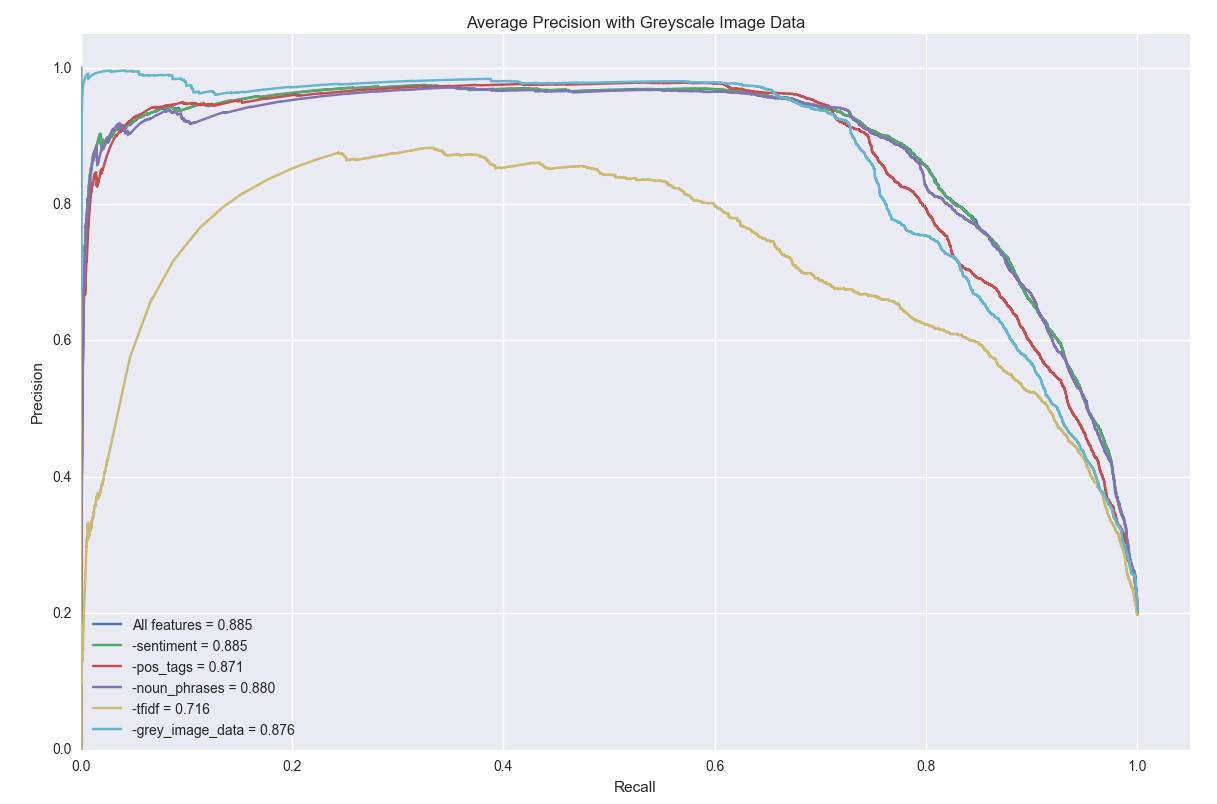
\includegraphics[width=0.75\textwidth]{greyscale_ablation.png}
\caption{Ablation analysis results using greyscale images as ``base'' feature set.}
\label{fig:grey}
\end{figure}

\begin{figure}[h]
\centering
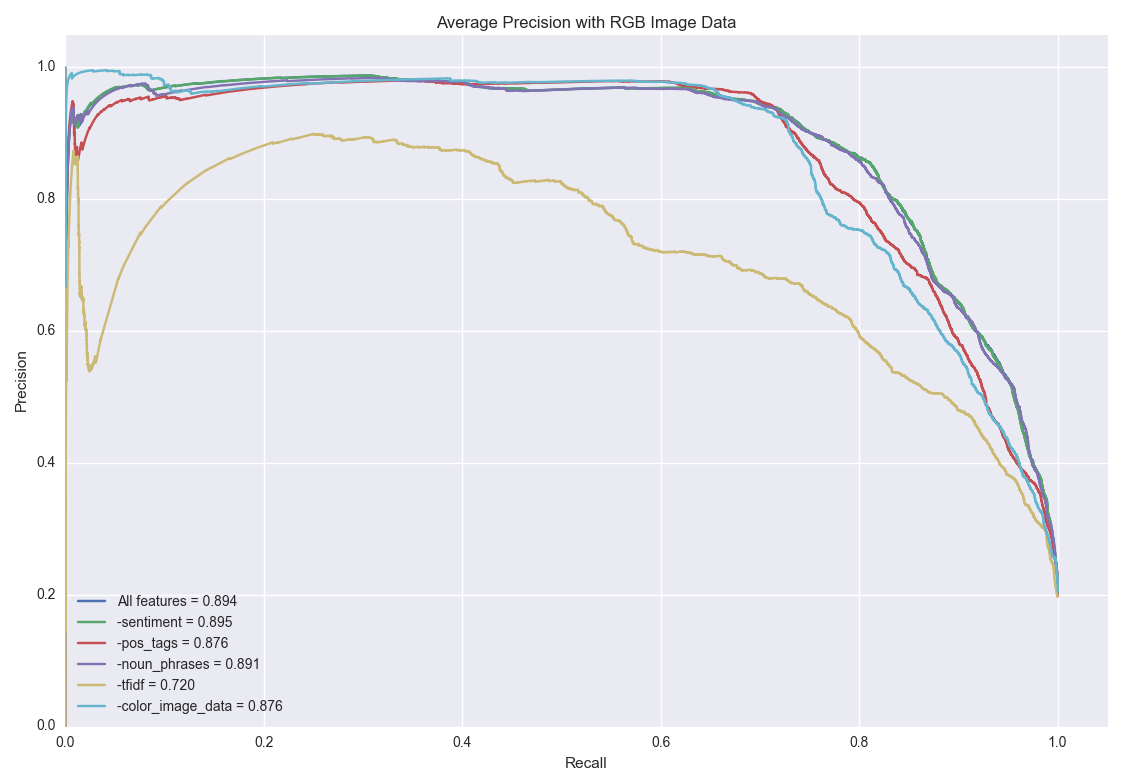
\includegraphics[width=0.75\textwidth]{RGB_ablation.png}
\caption{Ablation analysis results using RGB images as ``base'' feature set.}
\label{fig:rgb}
\end{figure}

\section{Discussion}
Given the use of somewhat noisy labels, the performance of the models tested in this work is impressive. In addition to outputting a final prediction for each instance in the test set, the linear SVM is also able to output a value quantifying its confidence that a particular instance belongs to either the positive or negative class.\footnote{Unlike logistic regression which outputs a probability as a confidence value, the linear SVM outputs a positive or negative real-valued number quantifying that particular instance's distance from the hyperplane. These values are used to rank the confidence values of the SVM for the images in this section.} These values were used to rank the images in order to inspect from a qualitative perspective the performance of the classifier in terms of top-ranked and bottom-ranked images. Intuitively, if the classifier is learning a reasonable signal for protest images, most of the top-ranked images should pertain to scenes of protest, while the bottom-ranked images should contain ``everything else.''
\par
Figures \ref{fig:top} and \ref{fig:bottom} show predictions with the highest and lowest rankings in terms of classifier confidence value. The images in Figure \ref{fig:top} show some reasonable predictions for images depicting protest scenes, although the author acknowledges that this is a somewhat subjective category for images. Overall, the vast majority of the top-ranked images show some type of scene depicting groups of people gathered and engaging in some type of protest or demonstration. One interesting mistake is the prediction of an ``I Can't Breathe'' sign as a member of the positive class. This is especially interesting given that the sign has primarily dark pixels, which calls into question whether the classifier is simply learning to separate light images from dark images.
\par
The bottom-ranked images in Figure \ref{fig:bottom} likewise provide some insight into model performance. Many of the images are lighter in shade, which seems to confirm the idea that a large part of what the classifier learns is to discriminate between light and dark images. However, there are also several darker images that show up in the bottom-ranked images, suggesting that the classifier is able to infer something more sophisticated in its predictions. Another interesting aspect about the bottom-ranked images is the prevalence of text and cartoons in these images. This suggests that one of the major decisions the classifier is making in the predictions is filtering out non-photographs from photographs. This is certainly useful, but calls into question what the classifier learns and whether this is a byproduct of the method of label extraction.

\begin{figure}[b]
\centering
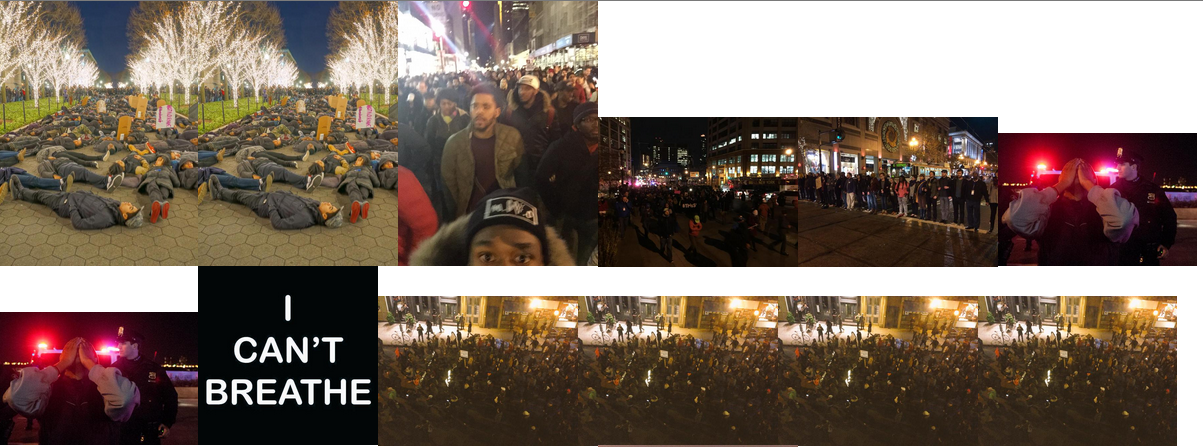
\includegraphics[width=0.75\textwidth]{top_ranked2.png}
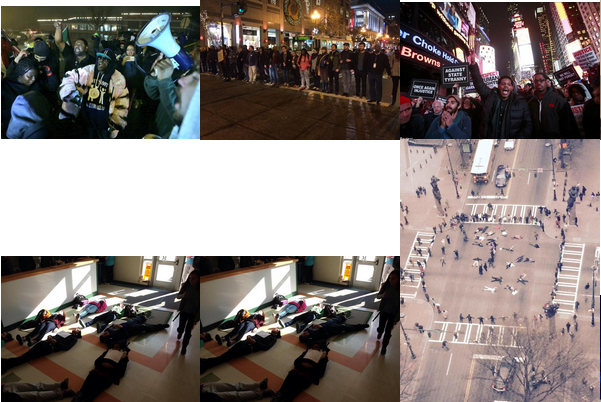
\includegraphics[width=0.75\textwidth]{top_ranked3.png}
\caption{Examples of top-ranked images according to the trained SVM.}
\label{fig:top}
\end{figure}

\begin{figure}[b]
\centering
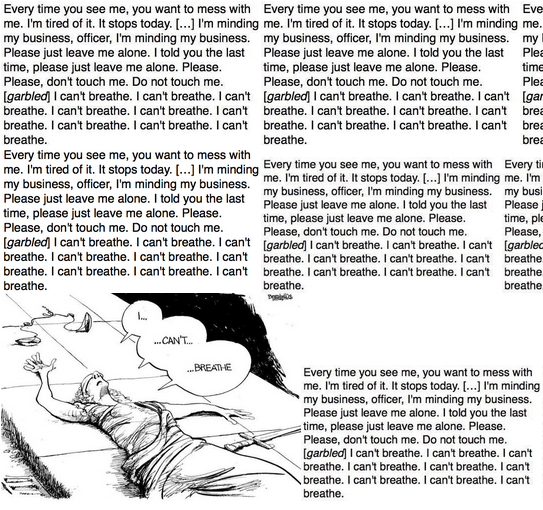
\includegraphics[width=0.75\textwidth]{bottom_ranked.png}
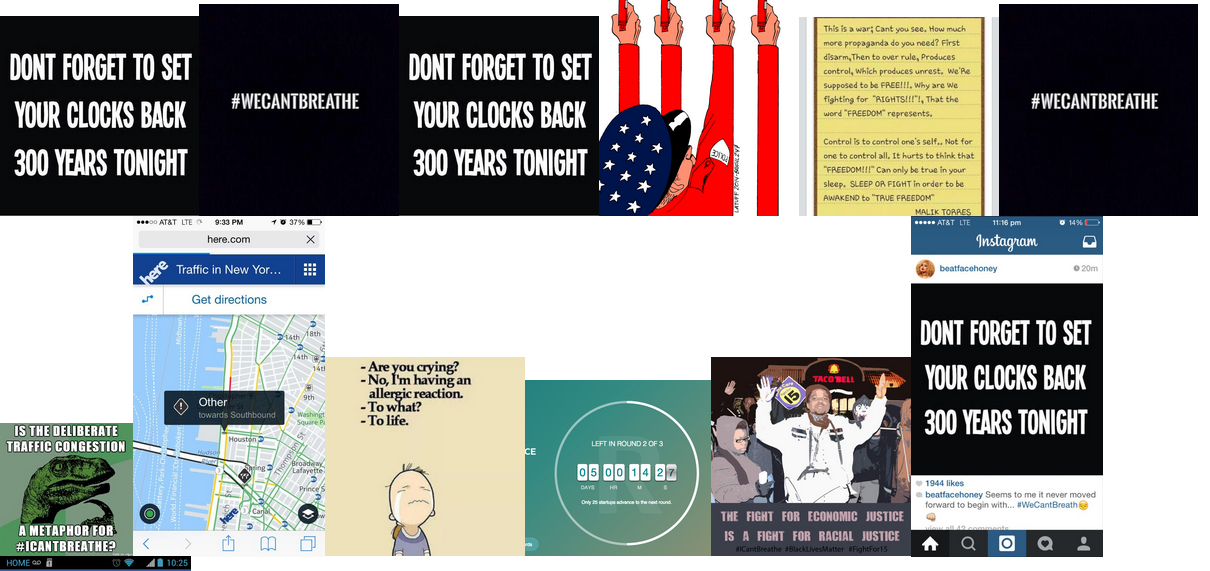
\includegraphics[width=0.75\textwidth]{bottom_ranked3.png}
\caption{Examples of bottom-ranked images according to the trained SVM.}
\label{fig:bottom}
\end{figure}

\section{Conclusion}
This project investigated the performance of SVM's in detecting protest scenes in images shared on Twitter. The results of this project show impressive performance in terms of average precision, and shows that linguistic features such as TF.IDF weighted unigram stems and part of speech are extremely helpful in this classification task. In addition, this project also sought to investigate the feasibility of automatically extracting labels from the text of tweets using straightforward natural language processing techniques. Initial qualitative results showed that this technique produces some noisy labels, but classifiers are still able to learn a reasonable signal with these labels.
\par
However, several open questions remain. One of the most straightforward is whether more sophisticated image features would aid in performance at this task. For this project, relatively simple global features were constructed in order to facilitate in scene recognition, however many other visual features could be explored for this task. Additionally, image data could be incorporated into the label extraction process as well to improve the quality of the labels. The text-based method seemed to work well for this initial set of experiments, however future work would likely benefit from using some kind of image similarity metric to construct the labels.
\par
Despite these shortcomings, this study sheds light on identifying protest scene images shared over social media from real events over a period of one week. While the dataset under analysis  stemmed from one particular event, the findings presented here are likely applicable to similar events as they play out over social media. The methods presented here could likely be applied to other data pertaining to events of social unrest, and could perhaps even be deployed through applications capable of real-time predictions and analysis. This could have profound effects for understanding these events as they unfold instead of having to study them in hindsight.

% Manual newpage inserted to improve layout of sample file - not
% needed in general before appendices/bibliography.

\label{app:theorem}

% Note: in this sample, the section number is hard-coded in. Following
% proper LaTeX conventions, it should properly be coded as a reference:

%In this appendix we prove the following theorem from
%Section~\ref{sec:textree-generalization}:

\bibliography{sample}

\end{document}